% *********************************************************************
% © 2024–2026 Jeremy Sylvestre
%
% Permission is granted to copy, distribute and/or modify this document
% under the terms of the GNU Free Documentation License, Version 1.3 or
% any later version published by the Free Software Foundation; with no
% Invariant Sections, no Front-Cover Texts, and no Back-Cover Texts. A
% copy of the license is included in the appendix entitled “GNU Free
% Documentation License” that appears in the output document of this
% PreTeXt source code. All trademarks™ are the registered® marks of
% their respective owners.
%
% *********************************************************************

\newcommand*{\xmin}{-0.5}
\newcommand*{\xmax}{8.5}
\newcommand*{\ymin}{-0.25}
\newcommand*{\ymax}{1.25}

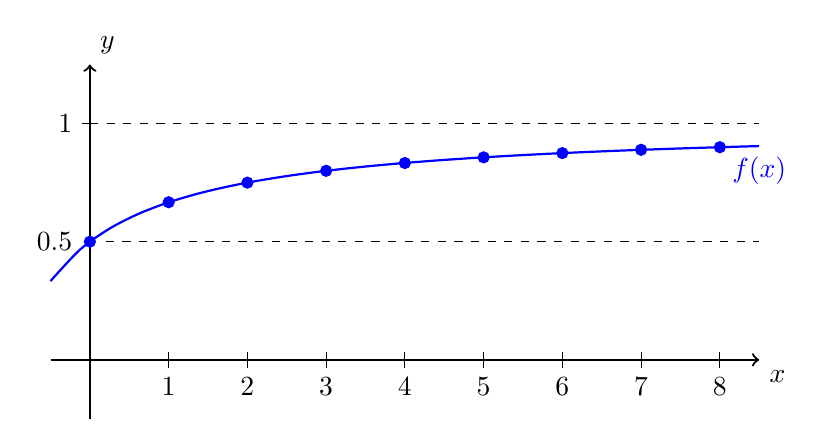
\begin{tikzpicture}
[
	closedpt/.style={circle,draw,fill,inner sep=0pt,minimum size=4pt},
	yscale=3
]

	% axis labels
	\foreach \x in {1,2,...,8} {
		\draw (\x,0.0333) -- (\x,-0.0333) node[below] {$\x$};
	}
	\draw (0.1,1) -- (-0.1,1) node[left] {$1$};
	\node[left] at (-0.1,0.5) {$0.5$};


	% axes
	\draw[->,thick] (\xmin,0) -- (\xmax,0) node[below right] {$x$};
	\draw[->,thick] (0,\ymin) -- (0,\ymax) node[above right] {$y$};

	% graph
	\draw[thick, blue, domain=-0.5:8.5,smooth] plot (\x,{(\x + 1) / (\x + 2)}) node[below] {$f(x)$};

	% upper/lower bounds
	\draw[dashed] (0,1) -- (\xmax,1);
	\draw[dashed] (0.2,0.5) -- (\xmax,0.5);

	% sequence
	\node[blue,closedpt] at (0,0.5) {};
	\node[blue,closedpt] at (1,0.667) {};
	\node[blue,closedpt] at (2,0.75) {};
	\node[blue,closedpt] at (3,0.8) {};
	\node[blue,closedpt] at (4,0.833) {};
	\node[blue,closedpt] at (5,0.857) {};
	\node[blue,closedpt] at (6,0.875) {};
	\node[blue,closedpt] at (7,0.889) {};
	\node[blue,closedpt] at (8,0.9) {};

\end{tikzpicture}
